\chapter{Rectangular Waveguide (3)}
%\begin{figure}
%\centering
%\includegraphics[width=1\linewidth]{\pathtoparttwo/graphics/Schematic-of-a-rectangular-waveguide-extending-along-z-a-and-the-TE10-top-and-TE11}
%\caption{}
%\label{fig:schematic-of-a-rectangular-waveguide-extending-along-z-a-and-the-te10-top-and-te11}
%\end{figure}
In the preceding chapter, we explored the electric field visualization within a parallel plane waveguide and delved into the modal characteristics of a rectangular waveguide. The identified mode as the \textbf{dominant mode of the rectangular waveguide} is the transverse electric mode with indices (1, 0), denoted as TE$_{10}$.

Emphasizing its significance, we operate predominantly in the TE$_{10}$ mode to mitigate dispersion, ensuring signal integrity both in the time domain and along the guided structure. Consequently, TE$_{10}$ becomes the primary focus during laboratory experiments and field applications.

This chapter focuses on examining the modal properties of TE$_{10}$, visualizing its fields, and calculating the waveguide's attenuation constant. Practical waveguides exhibit two types of losses: losses in the walls and losses in the dielectric medium.

The TE$_{10}$ mode's varying fields, derived from Equations~\eqref{eqn:te10start} to~\eqref{eqn:te10end}, are expressed as:
\begin{align*}
E_{x} &= E_{z} = H_{y} = 0\\
E_{y} &= \frac{-j\omega\mu a }{\pi} C\sin(\frac{\pi x}{a}) e ^{-j\beta z}\\
H_{x} &= \frac{j\beta a}{\pi} C \sin(\frac{\pi x}{a})e^{-j\beta z} \\
H_{z} &= C\cos(\frac{\pi x}{a}) e^{-j\beta z}
\end{align*}
The x and z component of the electric are zero and there is only a y component of the electric field. The x and z component of the magnetic field are non-zero and the y component of the magnetic field is zero. The variation of the fields is in the form of a sinusoid. In order to visualize the field we represent the fields as a real part of a complex quantity. So we can write the fields as
\begin{align}
\footnotemark\mathfrak{Re}\{E_{y}\} = A\sin(\frac{\pi x}{a})\sin(\frac{2\pi}{\lambda g}z)
\label{eqn:eyppw}\\
\mathfrak{Re}\{H_{x}\} = B\sin(\frac{\pi x}{a})\sin(\frac{2\pi}{\lambda g}z)\\
\mathfrak{Re}\{H_{z}\} = C\cos(\frac{\pi x}{a})\cos(\frac{2\pi}{\lambda g}z)
\end{align}
\footnotetext{
The j term is absorbed in the $e^{-j\beta z}$ term so that the real part of the field is taken.
}
where $A, B$ and $C$ are constants. The variation of these fields is illustrated in Figure~\ref{fig:lectureimage2}. Notably, $E_{y}$ is zero when $z = 0$, and it reaches maximum at $z = \frac{\lambda g}{4}$.

If we adjust the origin to $z = \frac{\lambda g}{4}$, then Figure~\ref{fig:lectureimage2} depicts the field variation. The electric field ($E_{y}$) is highest along the broader wall ($x = \frac{a}{2}$), and its variation resembles a sinusoidal pattern. The magnetic field lines ($H_{x}$ and $H_{z}$) form a loop, ensuring closure. 
\begin{figure}[h]
\centering
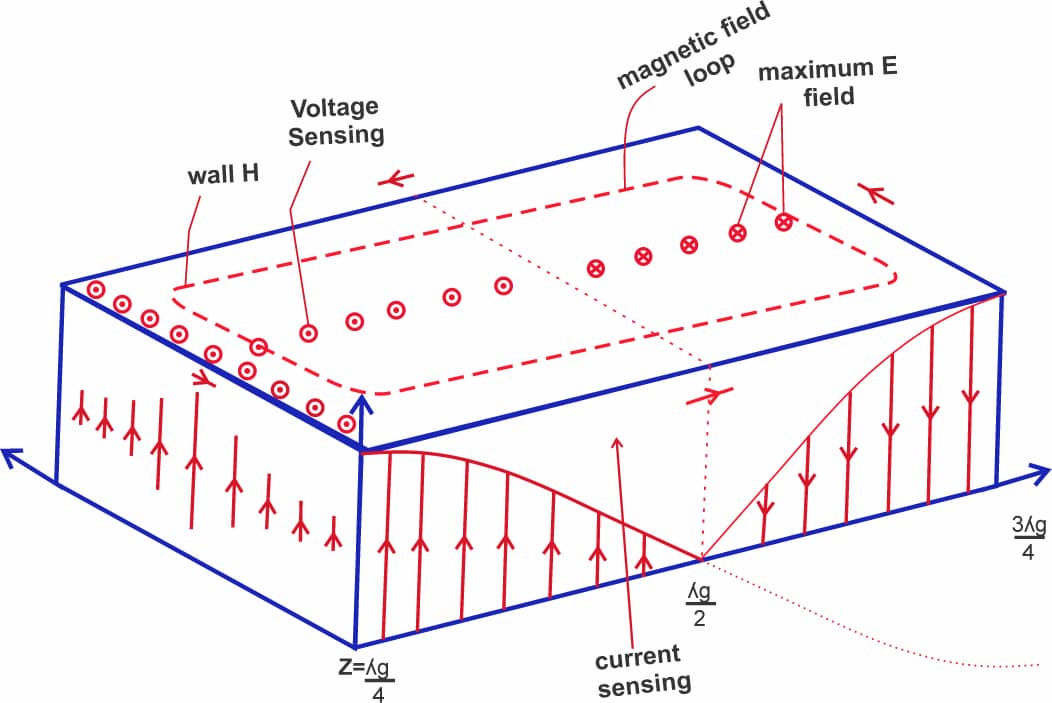
\includegraphics[width=1\linewidth]{\pathtoparttwo/graphics/lecture-image-2.jpg}
\caption{EM wave of a rectangular waveguide showing the field variations}
\label{fig:lectureimage2}
\end{figure}

$E_{y}$ reaches its maximum value with a sinusoidal variation along the $x$ direction, as indicated by the arrow lengths, all pointing in the positive $y$ direction for $x = 0$ to $x = a$. When observed from the top, this variation is represented by $\odot$ and $\otimes$, denoting the field direction. The size of the circles reflects the field strength. Sideways, the field exhibits a sinusoidal decrease, reaching zero at the edges.

In the plan view, the electric field and the x-component of the magnetic field are in phase its behaviour is illustrated at different $z$ positions in the end view, as depicted in Figure~\ref{fig:lectureimage3}.

\begin{figure}[h]
\centering
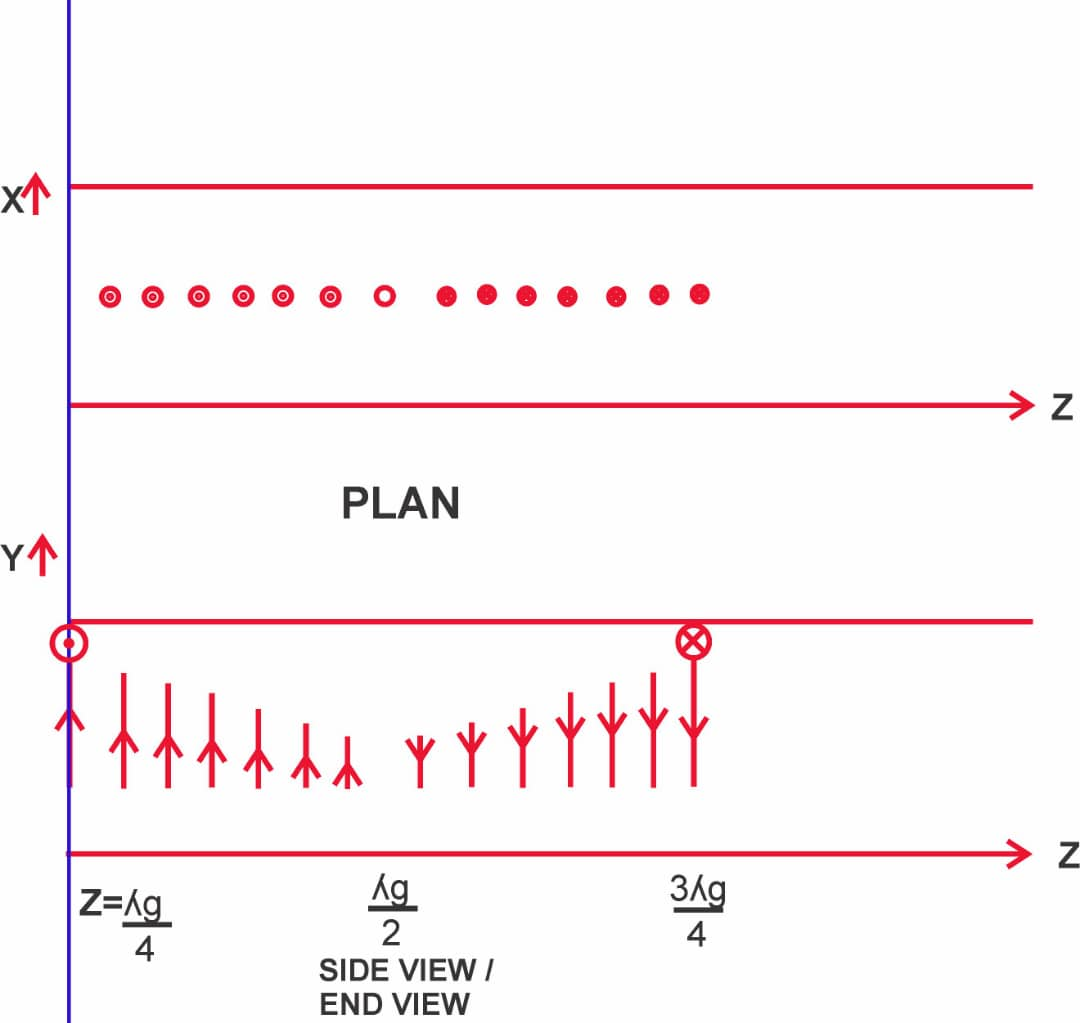
\includegraphics[width=1\linewidth]{\pathtoparttwo/graphics/lecture-image-3.jpg}
\caption{Plan and end view of an EM wave of a rectangular waveguide}
\label{fig:lectureimage3}
\end{figure}

As we have seen in the case of parallel plane waveguides, $H_{x}$ have variation the same as the electric field by $E_{y}$. $E_{y}$ and $H_{x}$ are maximum at the same point and minimum at the same point in space. But the z component of the magnetic field is shifted by $\pi/2$ or $\frac{\lambda g}{4}$ with respect to the x and z components. So wherever $H_{x}$ goes to zero, $H_{z}$ is maximum, so it is quadrature in x and z as we see in Figure~\ref{fig:lectureimage3}. Thus, we observe that;
\begin{align}
\mathfrak{Re}\{H_{x}\} = B\sin(\frac{\pi x}{a})\sin(\frac{2\pi}{\lambda g}z)\\
\mathfrak{Re}\{H_z\} = C\cos(\frac{\pi x}{a})\cos(\frac{2\pi}{\lambda g}z)
\end{align}

So where $H_{x}$ is maximum along z i.e  $z=\frac{\lambda g}{4}$, $H_{x}$ is minimum. The magnetic field lines are shown in Figure~\ref{fig:lectureimage1} with arrows designated 1, 2, 3 and 4\footnote{
Carefully observe $H_{x}$ and $H_{z}$ are maximum and where they occur.
}. So because the magnetic field must close on itself, 1, 2, 3, and 4 must form a loop as shown in Figure~\ref{fig:lectureimage2}. The variation of the magnetic field in the y-direction is zero. Hence $H_{x}$ and $H_{z}$ are constant in the y direction. So in the plan view, it appears as shown in Figure~\ref{fig:lectureimage2} with appropriate direction so that $E\times H$ gives the direction of propagation of the wave which is the z direction.

From the end view, at $z=\frac{\lambda g}{4}$ we have the magnetic field on the side wall coming out of the paper and at $z=\frac{\lambda g}{2}$, only $H_{z}$ is represented. At $z=\frac{3\lambda g}{4}$, we have $H_{x}$ going in the direction of $\otimes$. A three-dimensional representation of the fields is shown in Figure~\ref{fig:lectureimage4}. The electric field appears as rods, while the magnetic field resembles rolled carpets. This visualization aids in understanding how the fields can be excited and detected using voltage and current probes on the waveguide walls.
\begin{figure}[h]
\centering
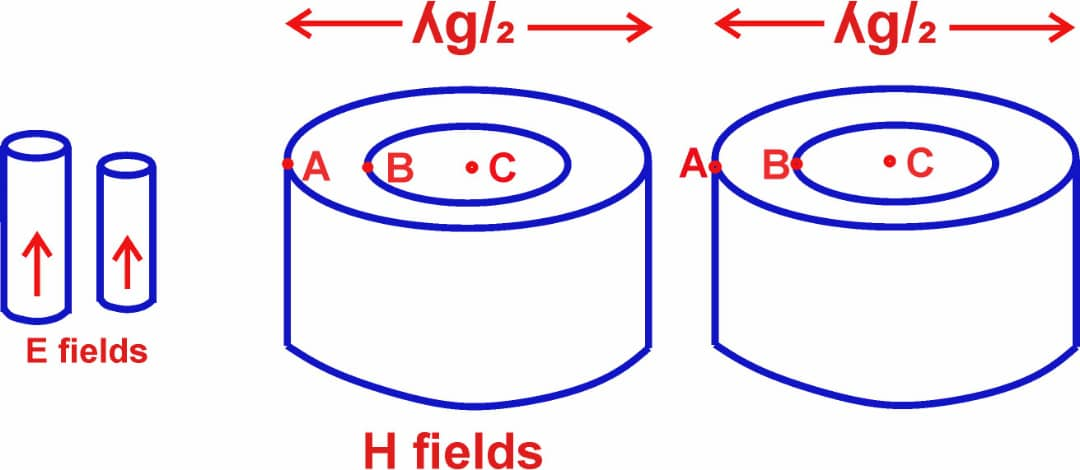
\includegraphics[width=1\linewidth]{\pathtoparttwo/graphics/lecture-image-4.jpg}
\caption{Representation of the field in three dimensions}
\label{fig:lectureimage4}
\end{figure}

After obtaining the field visualization at a specific instant, we consider letting this pattern move with the phase velocity inside the waveguide—essentially allowing the pattern to drift. At any location, we may observe patterns denoted as A, B, or C, as illustrated in Figure~\ref{fig:lectureimage4}. Notably, the electric field attains its maximum on the broader wall of the waveguide, as mentioned earlier.

For the TE$_{10}$ mode, the maximum electric field occurs along the broad wall at the plane $x = \frac{a}{2}$ as the wave travels in the z-direction. Simultaneously, the magnetic field achieves its maximum on walls G and H. Since it does not vary with $y$, if we need to excite the waveguide using electric fields with a voltage probe, the probe must be positioned on the line of the broader wall (i.e., $x = \frac{a}{2}$ middle point). This excites the electric field corresponding to TE$_{10}$. Conversely, for a current probe, it should be placed on the side walls of G and H to excite the field distributions we have visualized. This approach aids in exciting the TE$_{10}$ mode inside the waveguide. The same principle applies when the waveguide has specific modal properties, and we intend to sense the voltage and current on it. The voltage probe should be mounted on the broader wall, and the current probe should be on sidewalls G and H. This is how the fields inside a rectangular waveguide are detected using voltage and current probes or excited by providing signals to the probes protruding into the waveguides, thereby exciting a field within the structure.

The visualization of the field for the dominant TE$_{10}$ mode proves useful as it guides us on achieving field excitation by placing voltage and current probes on the waveguide walls. Understanding the field distribution in the TE$_{10}$ mode, with an electric field resembling a rod and a magnetic field akin to a rolled carpet or transformer stamping, facilitates the drawing of electric and magnetic fields for higher-order modes. For instance, if we wish to excite the TE$_{20}$ mode in the rectangular waveguide, we can leverage our understanding.

While we can write down the field expressions for electric and magnetic fields and visualize them similarly to TE$_{10}$, understanding that electric and magnetic fields follow a specific form allows us to stretch our imagination to visualize these fields for higher-order modes.

In the TE$_{20}$ mode, represented by the index 2, there are two cycles in the $x$ direction with no variation in the $y$ direction. Consequently, the electric field always lies in the $y$ direction. Concerning the magnetic fields, they resemble transformer stampings or rolled carpets, with two sections, each exhibiting a magnetic loop, as depicted in Figure~\ref{fig:lectureimage4}. The magnetic field's direction aligns with the Poynting vector in the $z$-direction. All fields essentially travel together in the region between the two magnetic loops, resembling two stacked rolled carpets in the TE$_{20}$ mode of the waveguide. Once a fundamental understanding of field visualization is established, it becomes straightforward to visualize fields for higher-order modes.

\section{Analysis of Surface Currents in Rectangular Waveguides}\index{surface current}
In the exploration of waveguide behaviour, a pivotal inquiry arises regarding the excitation of fields within the waveguide. Specifically, when these fields are energized, surface currents emerge within the waveguide. Again,  this analysis focuses on the TE$_{10}$ mode, where the surface current correlates with the tangential component of the magnetic field.

Consider the top and bottom walls of the waveguide depicted in Figure~\ref{fig:lectureimage5}. On these walls, the magnetic field alternates between the z and x directions, indicating a changing magnetic field direction. Conversely, the side walls consistently feature a magnetic field along the z-direction. Calculating the cross product of the unit normal vector ($\hat{n}$) and the magnetic field vector (H) for each wall yields the surface current direction.
\begin{figure}[h]
\centering
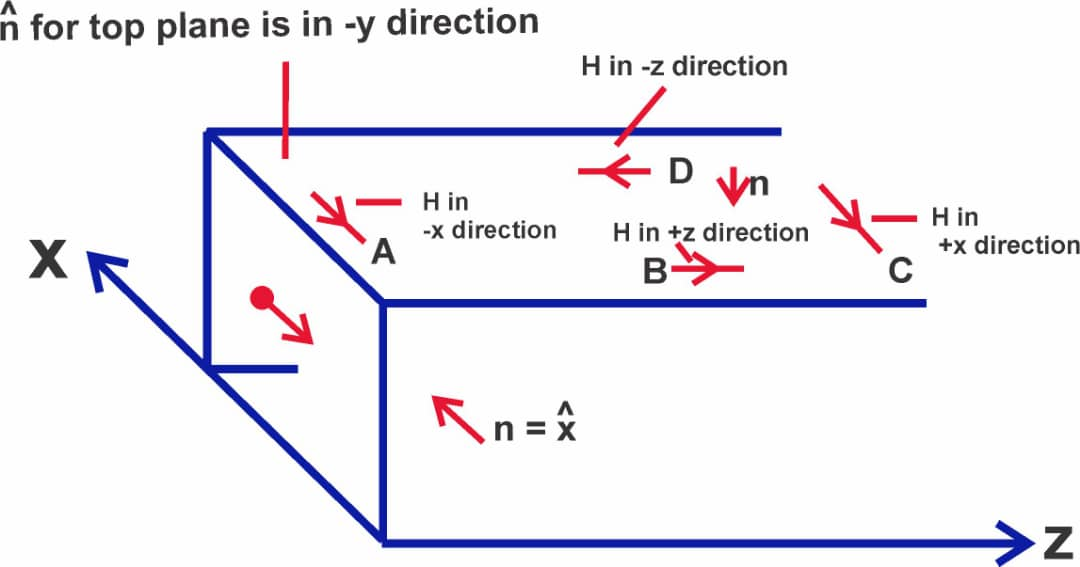
\includegraphics[width=1\linewidth]{\pathtoparttwo/graphics/lecture-image-5.jpg}
\caption{Direction of the surface current and magnetic field in a rectangular waveguide}
\label{fig:lectureimage5}
\end{figure}
\begin{figure}[h]
\centering
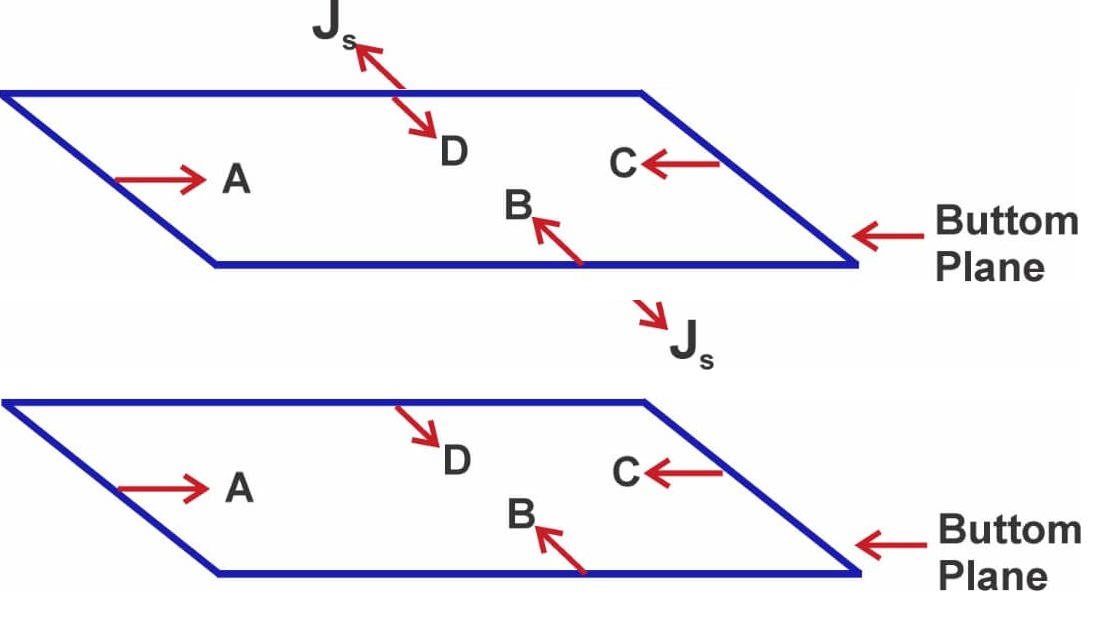
\includegraphics[width=1\linewidth]{\pathtoparttwo/graphics/lecture-image-6.jpg}
\caption{Direction of the surface current and magnetic field on the top and bottom walls of a rectangular waveguide}
\label{fig:lectureimage6}
\end{figure}

For instance, on the top surface, the current flows in the x and z directions, while on the side walls, it varies between the y direction as depicted in Figure~\ref{fig:lectureimage6}.

On the top wall, the cross product of $\hat{n}$ and H yields
\begin{dmath*}
\hat{n} \times H
= -\hat{y} \times (\pm\hat{x} \pm\hat{z})
= (-\hat{y} \times \pm\hat{x}) + (- \hat{y} \times \pm\hat{z})
= \pm\hat{z} \pm\hat{x}
\end{dmath*}
Hence we see the variation of $J_{s}$ on the top wall as it keeps changing direction.

For the right side wall, the magnetic field is in the z direction and for the left side wall, it is in the negative z direction. The cross product of $\hat{n}$ and H yields
\begin{align*}
\hat{n} \times H = \hat{x} \times \hat{z} = -\hat{y}\quad\text{for the right side wall}\\
\hat{n} \times H = -\hat{x} \times (-\hat{z}) = -\hat{y}\quad\text{for the left wall}
\end{align*}

This variation is visually depicted (see Figure~\ref{fig:surface_current_te10}), revealing a dynamic current distribution along the top surface and a constant direction along the side walls.

Examining the vertical walls, the surface current consistently flows in the y-direction due to the normal direction being in the x-direction and the magnetic field direction in the z-direction. Consequently, the current distribution across the four walls forms a pattern where the current appears to emanate from a point, flows along the top surface, remains constant along the side walls, and diminishes on the opposite surfaces.
	
This current phenomenon, resembling a blooming flower with alternating peaks and troughs, elucidates the induced currents in the rectangular waveguide oscillating every $\frac{\lambda_g}{2}$.
\begin{figure}[h]
\centering
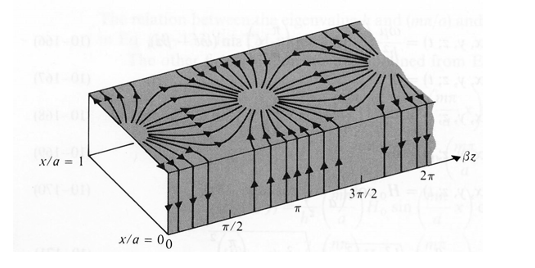
\includegraphics[width=1\linewidth]{\pathtoparttwo/graphics/surface_current_te10.png}
\caption{Surface current distribution on a rectangular waveguide}
\label{fig:surface_current_te10}
\end{figure}

Understanding these currents is essential for antenna design, as disruptions to the current flow through slots can impact radiation. Strategic placement of slots, aligned with the current flow, optimizes radiation efficiency.  So that there is a possibility of radiation, if we cut a slot that does not distort the current flows, as shown in Figure~\ref{fig:lectureimage10}.
\begin{figure}[h]
\centering
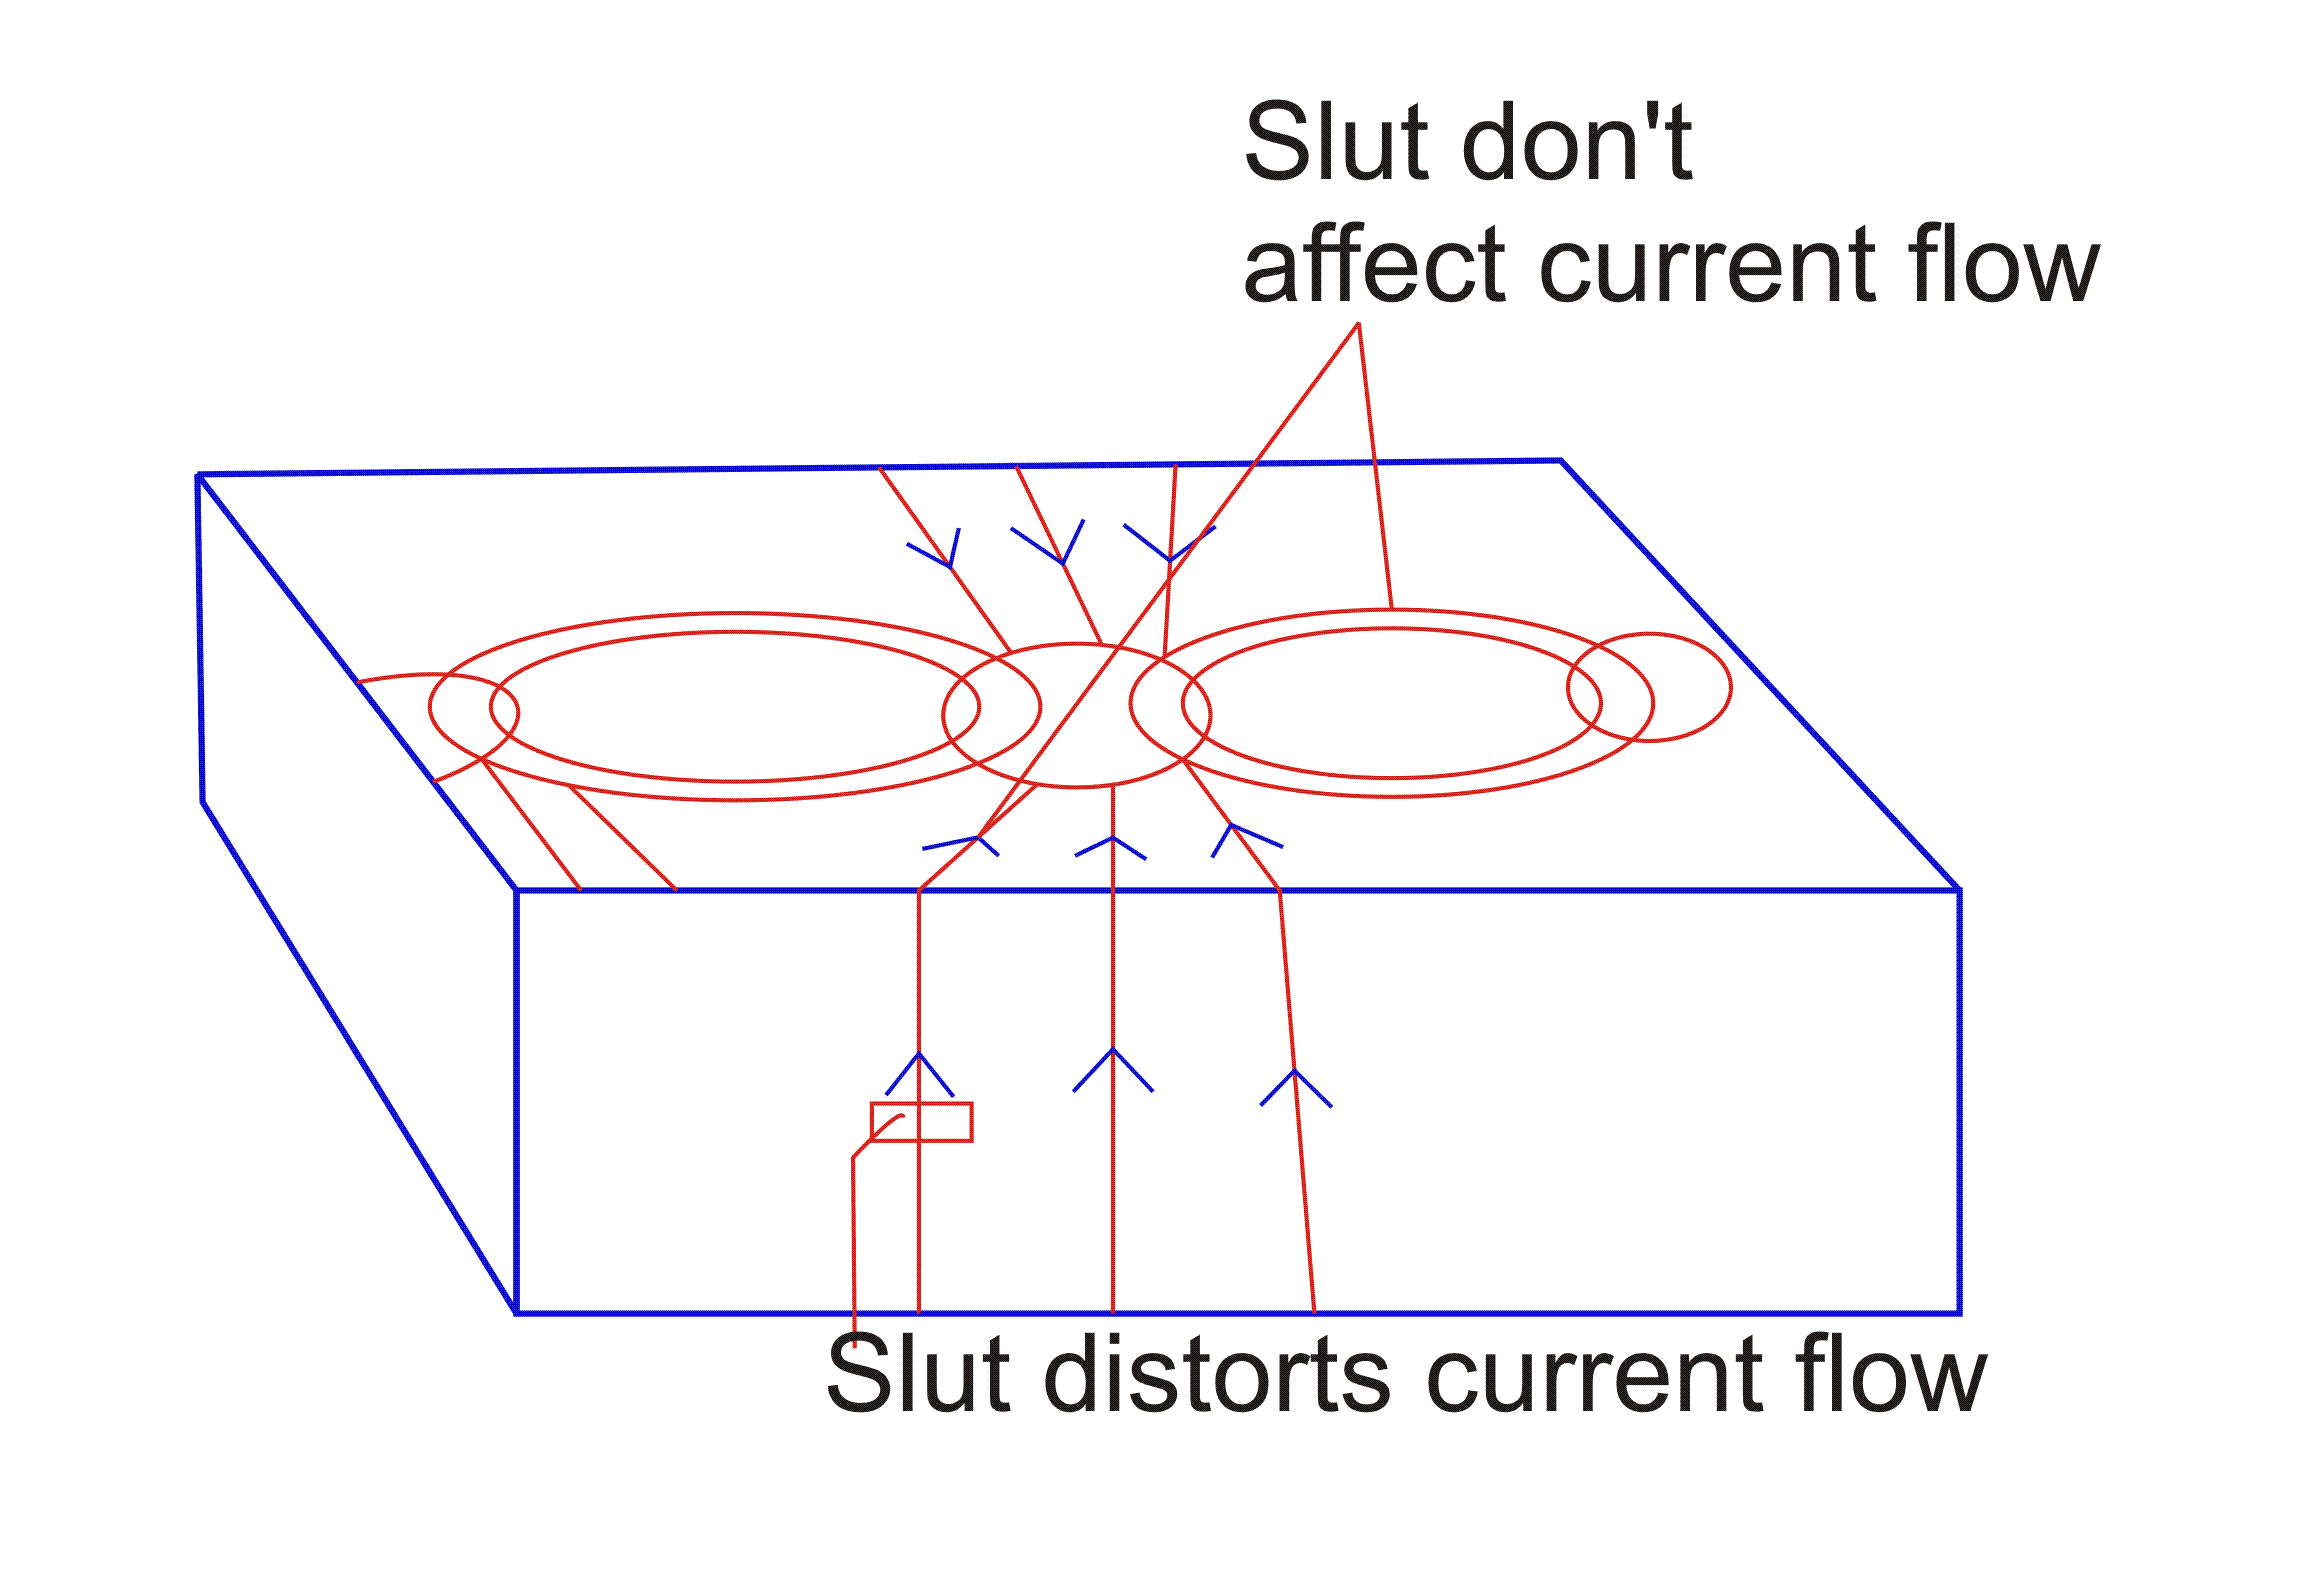
\includegraphics[width=1\linewidth]{\pathtoparttwo/graphics/lecture-image-10.png}
\caption{Diagram showing the relationship between slot openings and current flow}
\label{fig:lectureimage10}
\end{figure}

Moreover, awareness of current distribution aids in predicting losses within the waveguide. Non-ideal conductors along the walls introduce ohmic losses, influencing power propagation. Knowledge of current distribution thus becomes integral for both optimizing radiation and assessing losses in practical waveguide applications. This insight sets the stage for delving into the next critical aspect of waveguide analysis: calculating losses in a rectangular waveguide.

\section{Attenuation Constant}
In the pursuit of determining the loss per unit length in a rectangular waveguide, we turn our attention to a crucial parameter known as the \textbf{attenuation constant}\index{attenuation constant}. Analogous to its role in transmission lines, the attenuation constant $\alpha$ characterizes the exponential decay of fields along the structure, given by $e^{-\alpha z}$.

The task at hand involves finding the attenuation constant for the conductivity parameter of the walls and the loss in the dielectric if present. However, this endeavour is complicated due to the interaction between losses and field distributions in the waveguide. In the presence of losses, the electric and magnetic fields undergo modifications, and these changes impact the overall loss since it is intricately related to current distribution. Thus, a loop emerges: loss calculation requires knowledge of electric and magnetic fields, while the fields depend on the loss.

To simplify this complex problem, we assume that the primary function of the waveguide is to efficiently transfer energy. Consequently, efforts are made to minimize losses by using materials with high conductivity for the walls and a pure dielectric. Under this assumption, we treat losses as small deviations from the ideal case, enabling us to consider the fields in the same manner as lossless waveguides. This assumption breaks the loop, allowing us to calculate losses based on the known electric and magnetic fields.

The total attenuation constant $\alpha$ comprises two components: $\alpha_{d}$ for dielectric loss and $\alpha_{c}$ for conductor loss. When calculating $\alpha_{c}$, we assume $\alpha_{d} = 0$, and vice versa.
	
\subsection{Dielectric Attenuation constant}
In calculating  $\alpha_{d}$ we use the same approach we used for a transmission line. That is we calculate the propagation constant $\beta$ and from the dispersion relation, simply replace the dielectric constant with the dielectric constant of a lossy medium. From Equation~\eqref{eqn:dispersionrelatn}, considering a rectangular waveguide in TE$_{10}$ mode, we have
\begin{equation}
\footnotemark\beta_l^{2} = \omega^{2}\mu\epsilon_{l} -\left(\frac{\pi}{a}\right)^{2}
\label{eqn:dispersrelte10}
\end{equation}
\footnotetext{
We rewrite $\beta$ as $\beta_l$ to indicate that the propagation constant is for a lossy medium.
}
$\epsilon_{l}$ is the relative permittivity for lossy medium given as:
\begin{align*}
\epsilon_{l} = \epsilon_{o}\epsilon_{rl}
\end{align*}
But $\epsilon_{rl} = \epsilon_{r}(1-j\tan\delta)$ and $\tan\delta$ is the loss tangent. We substitute for $\epsilon_{l}$ in Equation~\eqref{eqn:dispersrelte10} so that
\begin{equation*}
\beta^{2}_{l} = \omega^{2}\mu\epsilon_{o}\epsilon_{r}(1-j\tan\delta)
\end{equation*}
\begin{dmath*}
\beta^{2}_{l} = \omega^{2}\mu\epsilon_{o}\epsilon_{r} - j\omega^{2}\mu\epsilon_{o}\epsilon_{r}\tan\delta
= \beta^{2} - j\beta^{2}\tan\delta\quad\text{since $\beta$ for lossless medium is $\omega\sqrt{\mu\epsilon}$}
\end{dmath*}
\begin{dmath}
\beta_{l} = (\beta^{2} - j\beta^{2}\footnotemark\tan\delta)^{\frac{1}{2}}
\simeq \beta - \frac{j\beta\tan\delta}{2}
\end{dmath}
\footnotetext{
$\tan\delta$ is usually small for a low-loss dielectric medium.
}
So we have a phase constant $\beta_{l}$ which has a real and imaginary part. The real part is $\beta$ whereas the imaginary part is the attenuation constant due to lossy dielectric filling the waveguide.

\begin{align}
\alpha_{d} = \frac{\beta\tan\delta}{2}
\label{eqn:alphad}
\end{align}
Recall in waveguide the variation along z is $e^{-j\beta z}$ so you need imaginary values of $\beta$ to give you attenuation. A real value would give oscillatory terms in $\cos\beta z$ and $\sin\beta z$ while an imaginary term such as $\alpha_d$ yeilds $e^{-j}(\frac{j\beta\tan\delta}{2})$, an exponentially decaying term.

We can simplify $\alpha_d$ further since we know that $\tan\delta = \frac{\sigma}{\omega\epsilon_{o}\epsilon_{r}}$, We substitute into Equation~\eqref{eqn:alphad} to get
\begin{dmath}
\alpha_{d} = \frac{\beta \frac{\sigma}{\omega\epsilon_\circ\epsilon_r}}{2}
= \frac{\beta^2 \frac{\sigma}{\omega\epsilon_\circ\epsilon_r}}{2\beta}
= \frac{\omega^2\mu\epsilon_\circ\epsilon_r\sigma}{2\beta\omega\epsilon_\circ\epsilon_r}
= \frac{\omega\mu\sigma}{2\beta}
\label{eqn:attenuationconst}
\end{dmath}
We can express $\alpha_d$ in terms of the cut-off frequency by considering the propagation constant of a lossless medium, $\beta$.

For lossless cases, 
\begin{equation*}
\beta = \sqrt{\omega^{2}\mu\epsilon-\left(\frac{m\pi}{a}\right)^{2}-\left(\frac{n\pi}{b}\right)^{2}}
\end{equation*}
But for TE$_{10}$ we have that cutoff frequency, $\beta = 0$, that is
\begin{equation*}
\omega^{2}_{c}\mu\epsilon = \left(\frac{m\pi}{a}\right)^{2}+\left(\frac{n\pi}{b}\right)^{2}
\end{equation*}
As such
\begin{dmath*}
\beta = \sqrt{\omega^{2}\mu\epsilon-\omega^{2}_{c}\mu\epsilon} = \omega\sqrt{\mu\epsilon}\sqrt{1-\left(\frac{fc}{f}\right)^{2}}
\end{dmath*}
Substituting for $\beta$ in the Equation~\ref{eqn:attenuationconst}
\begin{dmath*}	
\alpha_{d}=\frac{\omega\mu\sigma}{2\beta}= \frac{\omega\mu\sigma}{2\omega\sqrt{\mu\epsilon}\sqrt{1-\left(\frac{fc}{f}\right)^{2}}}
\end{dmath*}
Dividing the numerator and denominator by $\omega\sqrt{\mu\epsilon}$
\begin{dmath}
\alpha_{d} = \frac{\sigma\sqrt{\frac{\mu}{\epsilon}}}{2\sqrt{1-\left(\frac{fc}{f}\right)^{2}}}=\frac{\sigma\eta}{2\sqrt{1 - \left(\frac{fc}{f}\right)^{2}}}
\label{eqn:attenuationconst2}
\end{dmath}
where $\eta= \sqrt{\frac{\mu}{\epsilon}}$. Therefore, Equation~\ref{eqn:attenuationconst2} serves as the formula for the attenuation constant, where $f_c$ represents the cutoff frequency of the mode in question.

Given the dielectric constant of the medium and assuming a negligible loss tangent, meaning the losses in the medium are minimal, we can determine the attenuation constant $\alpha_{d}$ attributed to the finite conductivity of the dielectric medium. It is noteworthy that for two losses, the attenuation constant is directly proportional to the conductivity of the medium, and $\alpha_{d}$ is intricately linked to the cutoff frequency. When the frequency significantly exceeds $f_{c}$, the expression reduces to $\frac{\sigma\eta}{2}$, resembling the case of the transmission line. In the context of the transverse electromagnetic mode, $\frac{\sigma\eta}{2}$ represented the attenuation constant for the transmission line.

When considering lossy mediums in the unbound domain, we previously obtained a loss described by $\alpha = \frac{\sigma\eta}{2}$. However, in the rectangular waveguide, the dielectric loss now also depends on the proximity to the cutoff frequency. If the frequency is very close to the cutoff frequency, the term $\sqrt{1 - \left(\frac{f_c}{f}\right)^{2}}$ approaches zero, causing Equation~\eqref{eqn:attenuationconst2} to become significantly large. Consequently, dielectric loss becomes a function of frequency, a characteristic absent in the transverse electromagnetic mode where $\alpha_{d}$ solely depended on conductivity. Thus, $\alpha_{d}$ is not only proportional to the dielectric conductivity $\sigma$ but also varies with the distance from the cutoff frequency of a specific mode. As proximity to the mode's cutoff frequency increases, dielectric loss intensifies. By leveraging this equation, we can calculate one component of the attenuation constant, namely the dielectric attenuation constant $\alpha_{d}$.

\subsection{Conductor Attenuation constant}
The next component we aim to calculate is the finite conductivity of the boundary. Unlike the straightforward calculation of the dielectric attenuation constant, determining the attenuation due to finite conductivity poses a more intricate challenge. As the fields now reside within the waveguide, a mere modification of the propagation constant is insufficient. We must resort to fundamental principles to compute the attenuation constant.

In the presence of losses, the electric ($E$) and magnetic ($H$) fields vary with respect to the longitudinal direction $z$, denoted as ${\hat{E}}, {\hat{H}} \ \sim\ e^{-\alpha z}$, where $\alpha$ signifies the attenuation constant. The power, proportional to $|{\hat{E}}|^{2}$ or $|{\hat{H}}|^{2}$ (given that power is ${\hat{E}}\times{\hat{H}}$), exhibits a power density represented by $W\sim e^{-2\alpha z}$, indicating a decay with increasing $z$. 

Taking the derivative of power, $W$, with respect to $z$ yields:
\begin{dmath*}
\dv{W}{z}\sim-2\alpha e^{-2\alpha z} = -2\alpha W 
\end{dmath*}
The attenuation constant $\alpha$, in general, can be expressed as:
\begin{equation*}
\alpha = \frac{\dv{W}{z}}{2W}
\label{eqn:calcalpha}
\end{equation*}

Physically, $-\dv{W}{z}$ represents the rate at which power decreases in the direction of $z$ or in the direction of wave propagation, while $W$ signifies the total power carried by the structure. Now that the attenuation constant can be calculated using two quantities—namely, power loss per unit length $(-\dv{W}{z})$ along the waveguide, divided by two times the power carried by the waveguide—this relationship can be represented more generally as:
\begin{dmath}
\alpha = \frac{\textnormal{Power decrease / unit length}}{2\times \textnormal{Total power carried by the waveguide}}
\end{dmath}

To calculate the attenuation constant, we need to determine two quantities: power loss per unit length and the total power carried by the waveguide. This necessitates knowledge of the $E$ and $H$ fields within the waveguide, as well as the surface current in its walls. The surface current provides information about the loss, enabling the calculation of power loss per unit length in the waveguide. Additionally, the product of $E\times H$ yields the Poynting vector, and integration over the cross-sectional area of the waveguide provides the total power flowing inside the waveguide.

Thus, $W = \int\frac{1}{2}\mathfrak{Re}\{\bar{E}\times\bar{H^*}\}\cdot{da}$ represents the total power flowing in the waveguide. Once the surface current $J_{s}$ on these walls is known, power loss per unit area is given by half the surface resistance $R_s$ multiplied by $|J_{s}|^{2}$. Knowing the surface current, the loss per unit area can be calculated, and with the height of the waveguide known, the loss per unit length of the waveguide can be determined. With these two quantities in hand, Equation~\eqref{eqn:calcalpha} can be utilized to calculate the attenuation constant of this waveguide due to the finite conductivity of the walls.

In the subsequent chapter, by leveraging this basic definition of the attenuation constant, we will derive the attenuation constant for two modes. The first mode pertains to a parallel plane waveguide in the TEM mode—considered the simplest mode, providing insight into how to calculate this quantity. Subsequently, we will calculate the attenuation constant for a rectangular waveguide in the TE$_{10}$ mode.

\section*{Exercises}
\begin{ExerciseList}
\Exercise[label={ex411}]
What is the dominant mode in a rectangular waveguide, and why is it important?

\Exercise[label={ex412}]
How are the electric and magnetic fields visualized inside a parallel plane waveguide? And what are the field patterns for TE$_{10}$ mode in a rectangular waveguide?

\Exercise[label={ex413}]
What is the attenuation constant in a waveguide, and how is it related to loss in waveguides? How is the attenuation constant affected by dielectric losses and conductor losses? And how does the loss tangent affect the attenuation constant in dielectric-filled waveguides?

\Exercise[label={ex414}]
How is surface current induced in a rectangular waveguide? And what is the relationship between surface current and magnetic field direction on different walls of the waveguide?

\Exercise[label={ex415}]
How is the attenuation constant related to power loss and total power carried by the waveguide?
\end{ExerciseList}
